
% titlepage-demo.tex
\documentclass{beamer}

\usetheme{Boadilla}


\begin{document}


\begin{frame}[t]{Motivations}
\begin{center}

\includegraphics[width=6cm,height=3cm]{images/MED_overview.png}
\end{center}
\begin{itemize}
\item Massive number of videos are produced every day. 
\begin{itemize}
\item YouTube: 300 hours uploaded per minute, with 3 billion viewers a day.
\end{itemize}
\item Video need to be indexed, searched based on its content.
\item Many applications: 
\begin{itemize}
\item User demands: tutorial videos such as "\textbf{how to make a cake}", "\textbf{how to repair an appliance}".
\item Security purposes: filter out irrelevant content such as "\textbf{how to make a bomb}".

\end{itemize}

\end{itemize}
\end{frame}


%\begin{frame}[t]{Motivation (cont'd)}
%A real world application:	to restrict violent video clips
%	\begin{center}
%		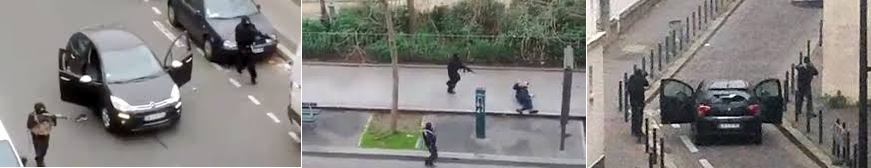
\includegraphics[width=11cm,height=2cm]{images/part1/charlie_hebdo_attacks.png}
%		\\
%		Footage of the Charlie Hebdo Attack (Paris - Jan 2015)
%	\end{center}
%	\begin{center}
%		
\includegraphics[width=6cm,height=3.5cm]{images/part1/facebook.png}
%		\\
%		Facebook has begun placing warnings over videos posted to its site
%	\end{center}
%\end{frame}

\begin{frame}[t]{Motivations (cont'd)}
A real world application: \textbf{detect shoplifting} (``manbiki'').

\begin{itemize}
	\item Jan, 2015: National manhunt in Japan for a YouTuber who allegedly stole...snacks [Mainichi News].
\end{itemize}
	\begin{center}
		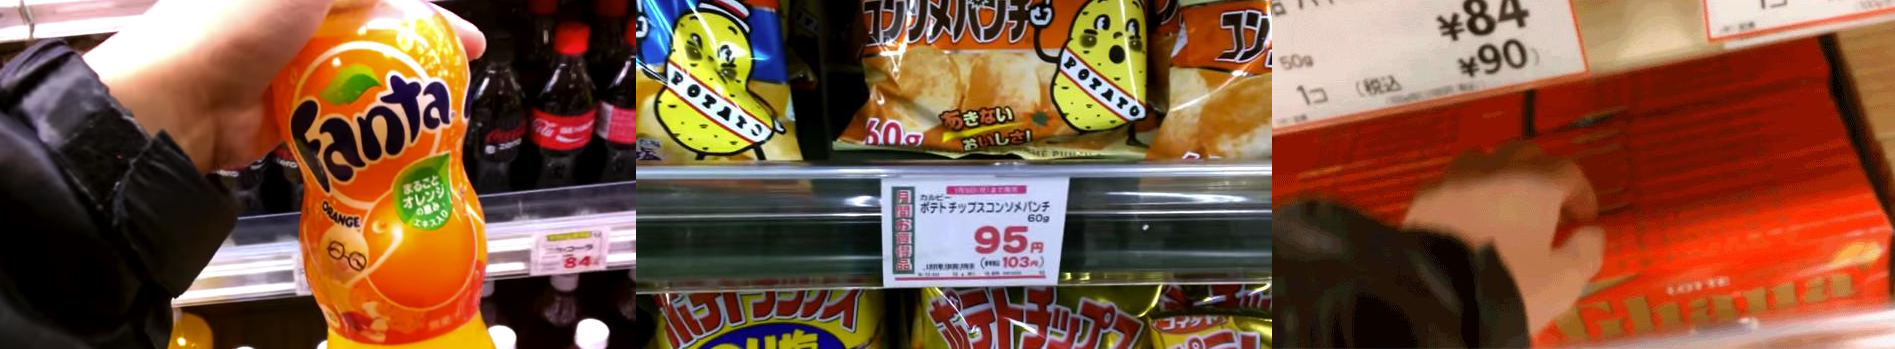
\includegraphics[width=11cm,height=2cm]{images/part1/snacks.png}
		\\
		The footage shows that he's stolen many things. 
	\end{center}
\begin{itemize}
	\item How can the police know? 
	\begin{itemize}
\item Because he has been uploading clips of his alleged thefts.
	\end{itemize}
	\item Can it be \textbf{automatically} detected by security cameras? 
\end{itemize}
\begin{tikzpicture}[remember picture,overlay]  
\node [xshift=-1.3cm,yshift=-7.5cm] at (current page.north east)
{
\includegraphics[width=2cm,height=2cm]{images/part1/conan.jpg}};
\end{tikzpicture}

\end{frame}


\begin{frame}[t]{Complex Event}
	\begin{definition} 
		\begin{itemize}
		\item is a complex activity occurring at a specific place and time;
		\item involves people interacting with other people and/or objects;
		\item consists of a number of human actions, processes and activities.
		\end{itemize}
	\end{definition}
	\begin{center}
	\begin{figure}
		\centering
		\begin{minipage}{.3\textwidth}
			\centering
			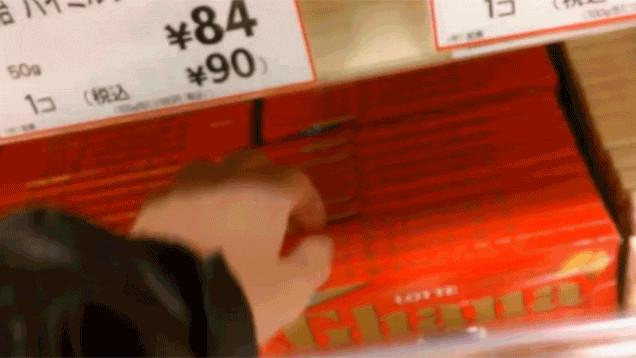
\includegraphics[width=1\linewidth]{images/part1/shoplifting1.jpg}
			\\
			\tiny{Pick up an item}
		\end{minipage}%
		\begin{minipage}{.3\textwidth}
			\centering
			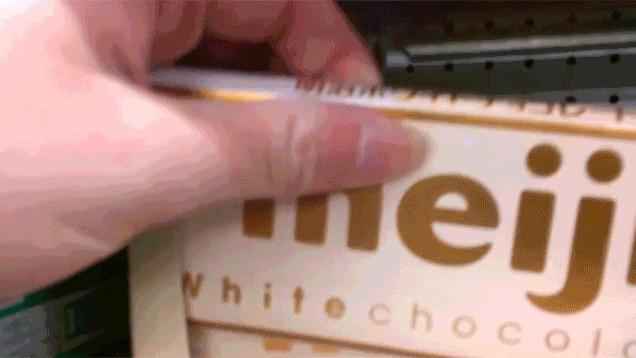
\includegraphics[width=1\linewidth]{images/part1/shoplifting2.jpg}
			\\
			\tiny{Keep it in a hidden place}
		\end{minipage}
		\begin{minipage}{.3\textwidth}
			\centering
			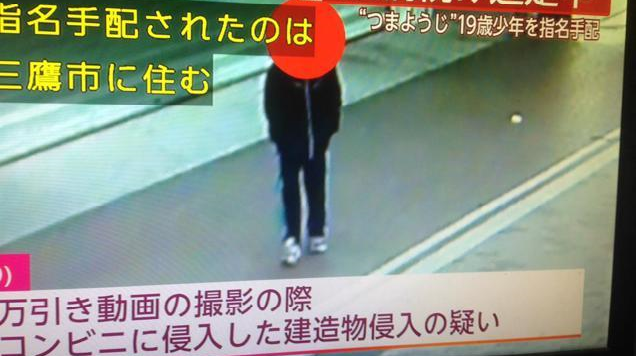
\includegraphics[width=1\linewidth]{images/part1/shoplifting3.jpg}
			\\
			\tiny{Get out successfuly}
		\end{minipage}
\footnotesize{Sequence of actions in the shoplifting event.}
	\end{figure}

	\end{center}
\small{Compared to \textbf{single action} detection [KTH dataset]}
	\begin{center}
		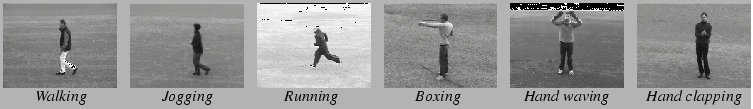
\includegraphics[width=11cm,height=1.6cm]{images/part1/kth.png}
	\end{center}
\end{frame}


\begin{frame}[t]{Event Detection from Video}
In 2010 TRECVID proposed Multimedia Event Detection (MED) task.
\begin{definition}
\begin{itemize}
\item Given: An event kit which consists of an event name, definition, explication + video example.
\item Wanted: A system that can search for this event through the large set of videos with reasonable accuracy and speed.
\end{itemize}
\end{definition}
\begin{center}
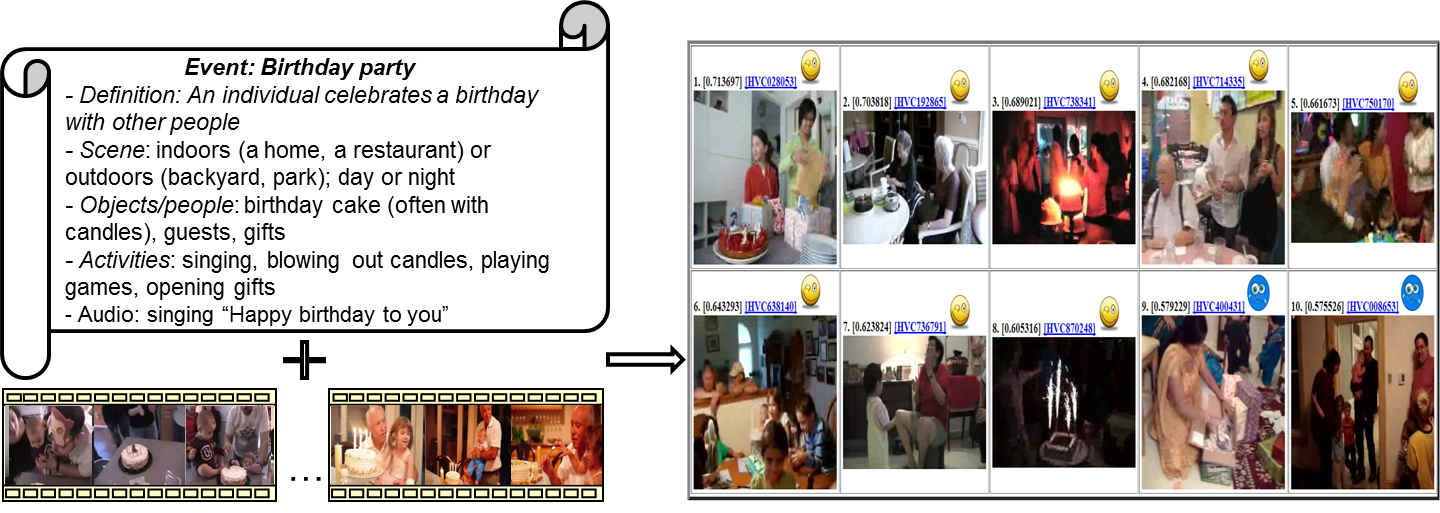
\includegraphics[width=12cm,height=4cm]{images/med_definition.png}
\end{center}


\end{frame}

\begin{frame}[t]{Challenges of Event Detection from Video}
	\begin{itemize}
		\item \textbf{Large content variation}: the diversity of complex
		event is very high.
	\end{itemize}
\begin{center}
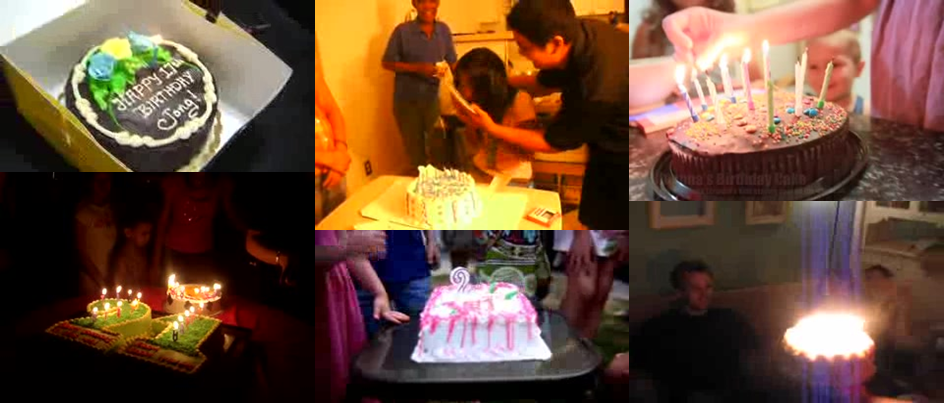
\includegraphics[width=10cm,height=4.5cm]{images/part1/largevariation.png}
\\
The large variation of \textit{birthday cake} in the ``birthday party'' event.
\end{center}
\end{frame}


\begin{frame}[t]{Challenges of Event Detection from Video (cont'd)}
	\begin{itemize}
		\item \textbf{Uncontrolled capturing conditions}: different time, location, clutter in the environment, camera motion $\rightarrow$ can contain irrelevant information to the event of interest.
	\end{itemize}
	\begin{center}
		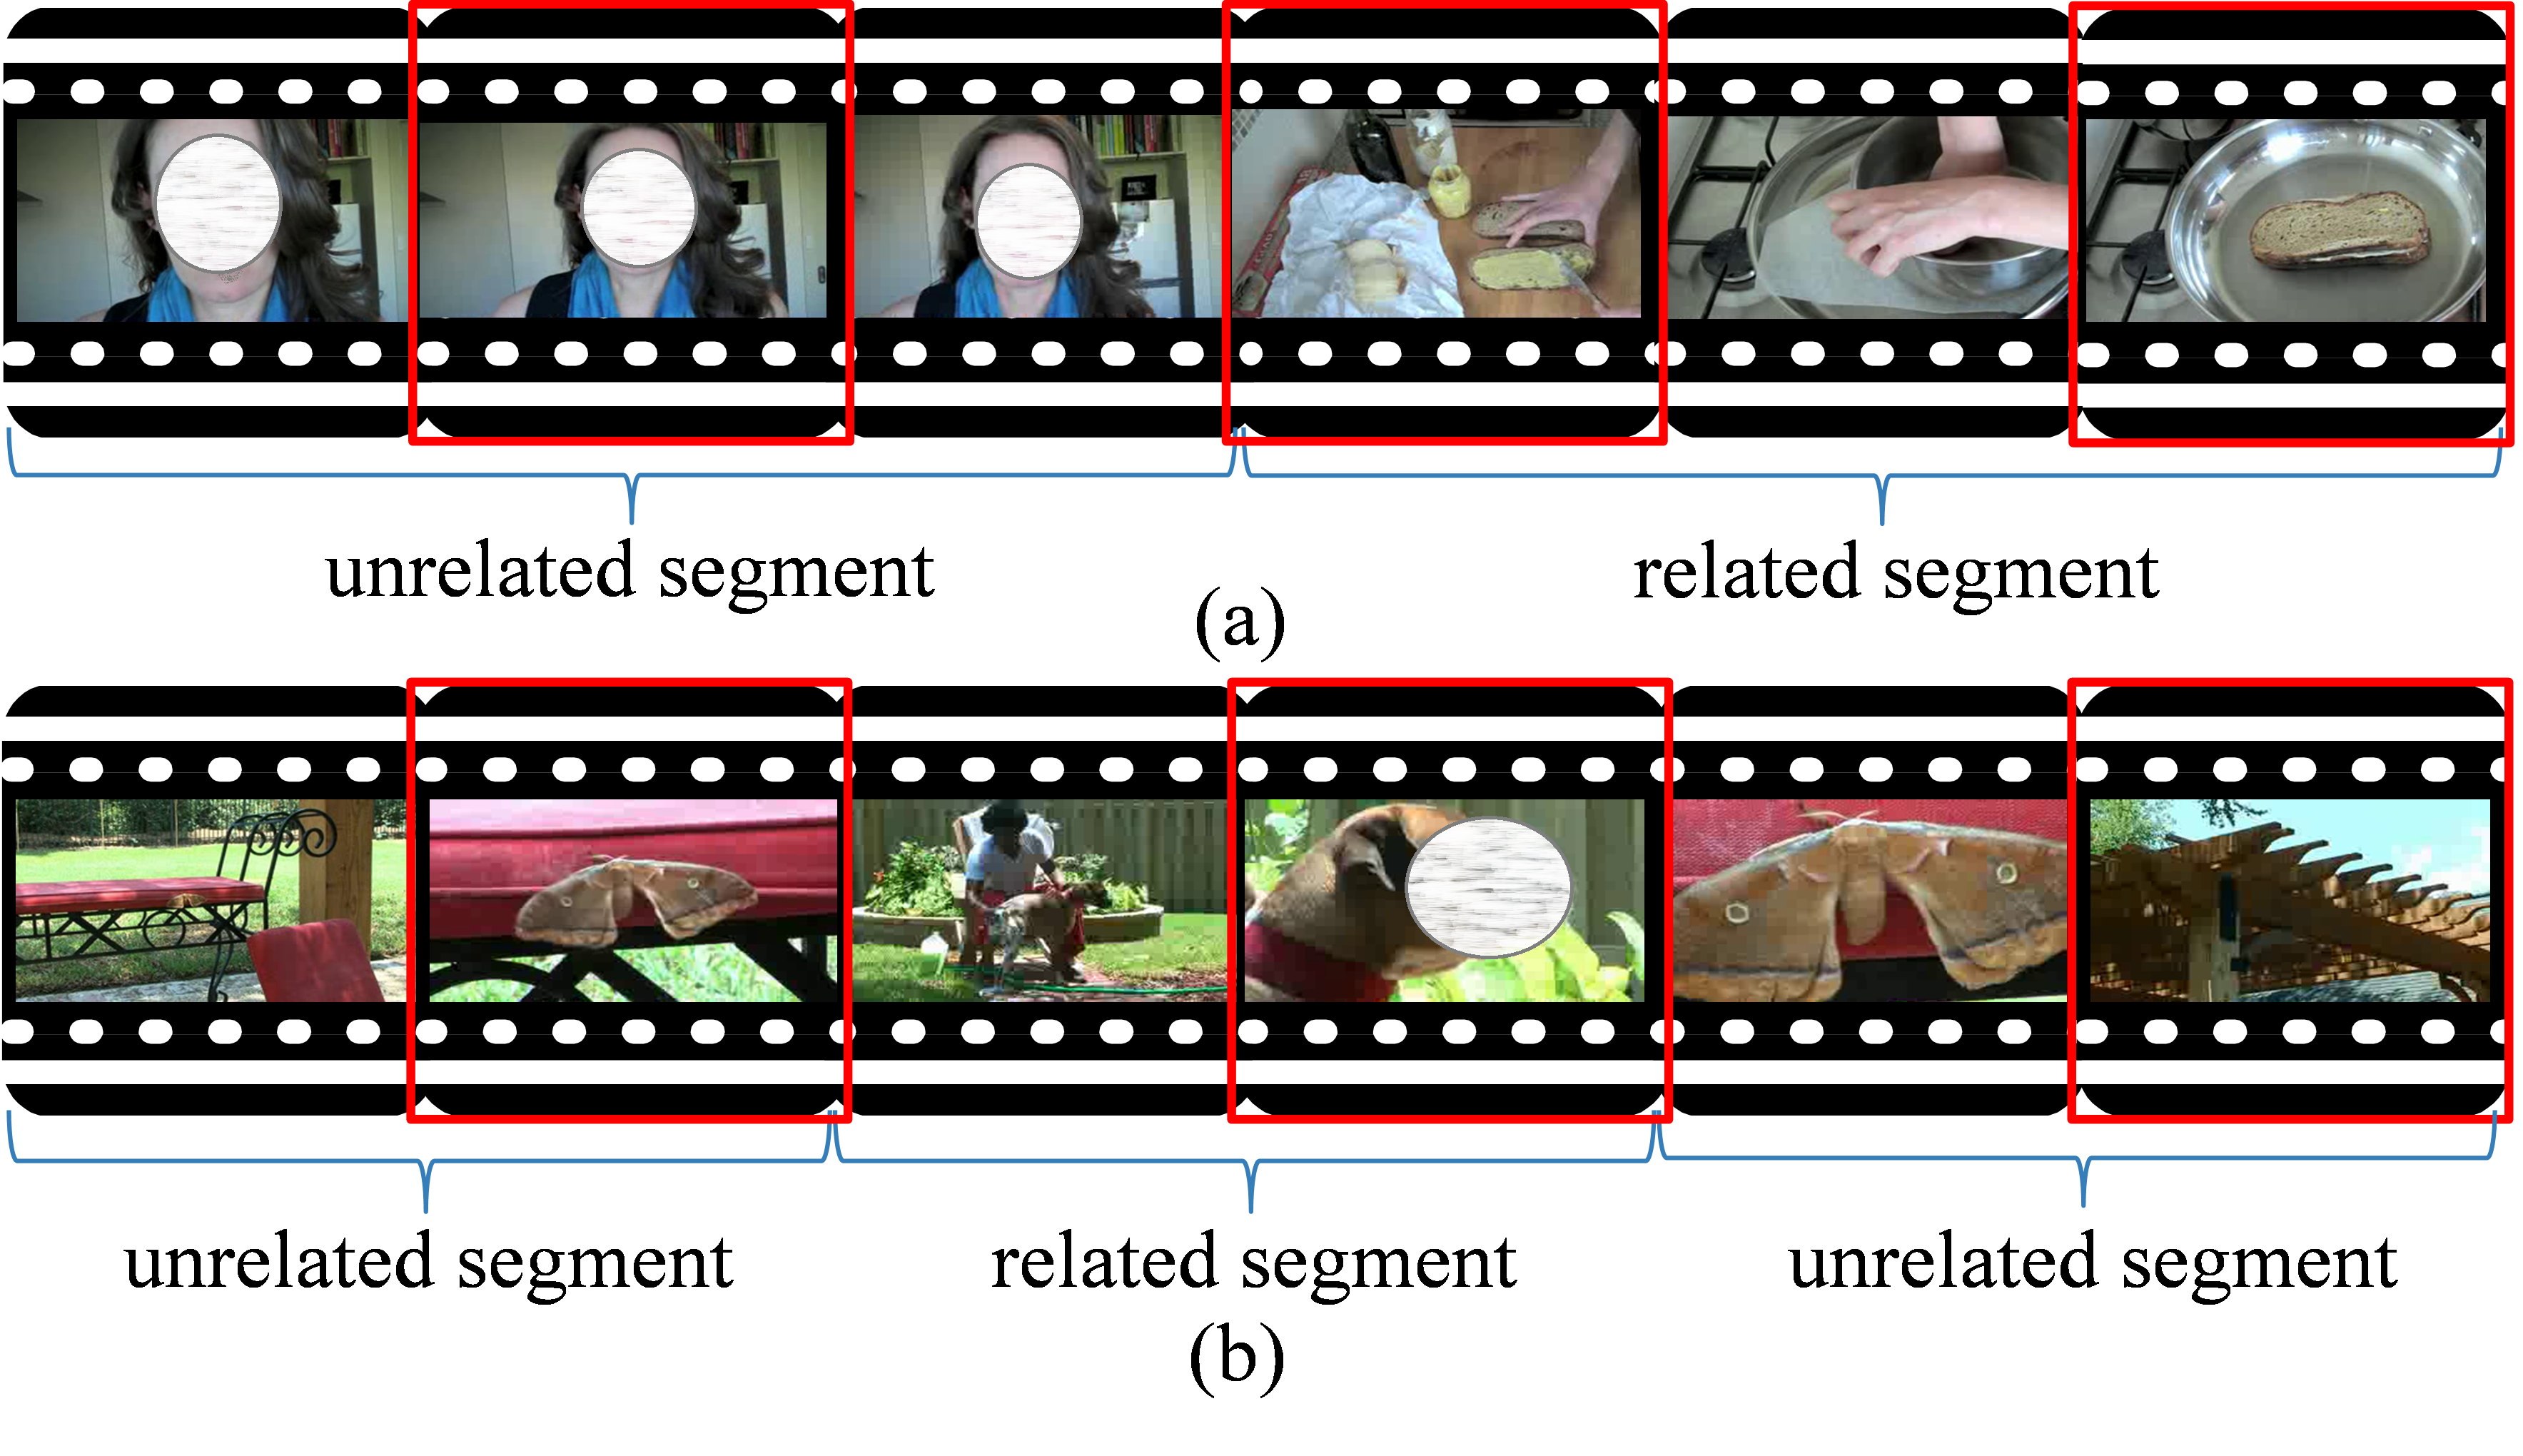
\includegraphics[width=10cm,height=5cm]{images/part1/uncontrolled.png}
		\\
		\footnotesize{(a) Example video for ``making a sandwich'' event: the related segment appears after a self-cam segment (unrelated); (b) example video for ``grooming an animal'' event: related segment is sandwiched between two unrelated segments.}
	\end{center}
	
\end{frame}


\begin{frame}[t]{Challenges of Event Detection from Video (cont'd)}
	
	\begin{itemize}
		\item Presence of \textbf{near-miss} (related) videos.
			\begin{itemize}
	\item closely related to the event but it lacks critical evidences to be a positive event instance.
			\end{itemize}
	\end{itemize}
	
	\begin{center}
		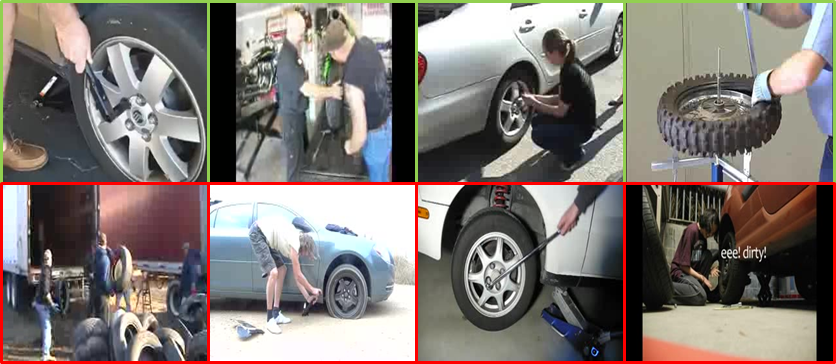
\includegraphics[width=10cm,height=4.5cm]{images/part1/nearmiss.png}
		\\
			\footnotesize{Example of \textit{near-miss} videos for ``Changing a vehicle tire'' event (2\textsuperscript{nd} row).}
	\end{center}
\end{frame}

\begin{frame}[t]{Challenges of Event Detection from Video (cont'd)}
\begin{itemize}
\item Large scale video archives
\end{itemize}
%\begin{tabular}{ | p{2cm} | p{2.5cm} | p{3cm} | p{3cm} | }
%\hline
%	Dataset & MED 2010 & MED 2011 & MED 2012  \\ \hline
%	Number of test events & \textbf{3} (Assembling a shelter, Batting a run, Making a cake) & \textbf{10} (Birthday party, Changing a vehicle tire, Flashmob gathering, etc) & \textbf{20} (Cleaning an appliance, Dog show, Marriage proposal, etc)  \\ \hline
%	Number of videos & \textbf{3,468} (1,744 dev videos and 1,724 test videos) & \textbf{45,000} (13,200 dev videos and 31,800 test videos) & \textbf{156,000} videos (58,000 dev videos and 98,000 test videos) \\ \hline
%	Number of background videos & \textbf{1,500} for dev and \textbf{1,500} for test & \textbf{10,000} for dev and \textbf{28,000} for test & \textbf{10,000} for dev and \textbf{95,000} for test \\ \hline
%	Hours of video & \textbf{110} & \textbf{1,400} & \textbf{4,850} \\ \hline
%\end{tabular}

\begin{table}[h]
	\centering
		Number of videos in the TRECVID MED collection up to 2014.
	\scriptsize
	\begin{tabular}{@{}|c|l|c|c|@{}}
		\toprule
		\multicolumn{2}{|c|}{Set}                                                                         & Number of video clips & Video duration (hours) \\ \midrule
		\multirow{3}{*}{\begin{tabular}[c]{@{}c@{}}Development\\ Data\end{tabular}}    & RESEARCH         & 10,000                & 314                    \\ \cmidrule(l){2-4} 
		& 10 Event Kits    & 1,400                 & 74                     \\ \cmidrule(l){2-4} 
		& Transcription    & 1,500                 & 45                     \\ \midrule
		\multirow{2}{*}{\begin{tabular}[c]{@{}c@{}}Event\\ Training Data\end{tabular}} & Event Background & 5,000                 & 146                    \\ \cmidrule(l){2-4} 
		& 40 Event Kits    & 6,000                 & 270                    \\ \midrule
		\multirow{2}{*}{Test Data}                                                     & MEDTest          & 27,000                & 849                    \\ \cmidrule(l){2-4} 
		& KindredTest      & 14,500                & 687                    \\ \midrule
		\multirow{2}{*}{Evaluation Data}                                               & MED14Eval-Full   & 198,000               & 7,580                  \\ \cmidrule(l){2-4} 
		& MED14Eval-Sub    & 33,000                & 1,244                  \\ \midrule
		\multicolumn{2}{|c|}{\textbf{Total}}                                                                       & \textbf{244,000}               & \textbf{9,911}                  \\ \bottomrule \bottomrule
		
				\multicolumn{2}{|c|}{\textbf{THUMOS14 (largest action dataset)}}                                                                       & \textbf{13,000}               & \textbf{254}                  \\ \bottomrule
	\end{tabular}
	\label{c2_dataset}
\end{table}

\end{frame}


\begin{frame}[t]{Target Challenge \& Research Direction}
	\begin{itemize}
		\item Target challenge: \textit{\textbf{Uncontrolled capturing conditions}} 
			\begin{itemize}
				
\item contains irrelevant information to the event of interest.
\item differentiates real video from studio/controlled-capturing video.
		 	\end{itemize}
		\item Research direction: Decompose the video into sub-sequences and study event detection methods from these sub-sequences.
	\end{itemize}
	\begin{center}
		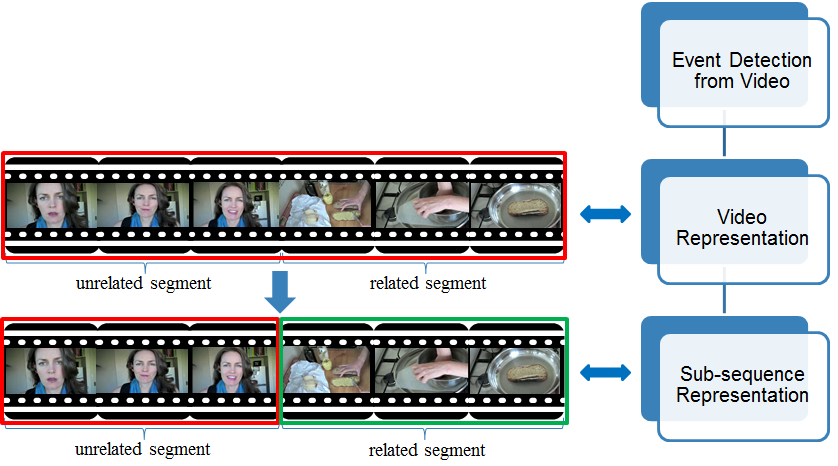
\includegraphics[width=10cm,height=5.5cm]{images/part1/mainchallenge.png}
		\\
		\footnotesize{}
	\end{center}
	
\end{frame}


\begin{frame}[t]{Contributions}
	
	\begin{enumerate}
		\item Segment-based \textbf{Representation} (SB)
		\begin{itemize}
			\item Investigate different strategies to \\
			decompose a video into segments.
			\item Study the optimal segment length.
		\end{itemize}
		\item Sum-Max Video \textbf{Aggregation} (SM)
		\begin{itemize}
			\item An efficient method to aggregate\\
			local features into video feature \\
			representation.
		\end{itemize}
		\item Event-driven Multiple Instance \\
				\textbf{Learning} (EDMIL)
		\begin{itemize}
			\item A method to leverage the event\\
			 description to learn key evidences \\
			 for complex event detection.
		\end{itemize}
	\end{enumerate}
	
\begin{tikzpicture}[remember picture,overlay]  
\node [xshift=-3cm,yshift=-4.5cm] at (current page.north east)
{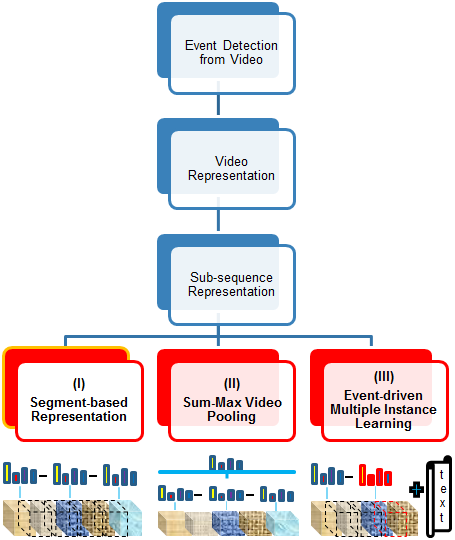
\includegraphics[width=5cm,height=7.5cm]{images/part1/contribution2.png}};
\end{tikzpicture}

\end{frame}

\end{document}